\section{Container vs virtuelle Maschinen}
\label{sec:container_vs_virtual_machines}
Wie in \autoref{subsec:soa} beschrieben, waren die durch die Installation von Services mitgebrachten, kumulativen Kosten einer der Gründe des Scheiterns von SOA. Zu jener Zeit musste für jeden Service Hardware eingekauft werden, auf welcher dieser Service installiert werden konnte. Wie in \autoref{subsec:microservices} beschrieben, bilden Microservices anhand des Single-Responsibility-Prinzips nur einen kleinen Teilbereich in dem Geschäft ab und sind somit feingranularer als durch SOA entworfene Services. Microservices bedeuten also automatisch mehr Services im Vergleich zu SOA und gleichzeitig mehr Server, auf denen die Microservices installiert werden müssen.

Sowohl virtuelle Maschinen als auch Container bieten eine Form der Virtualisierung, um Software installieren und bereitstellen zu können. Dabei benutzen beide Varianten unterschiedliche Ansätze, um dieses Ziel zu erreichen. In \autoref{fig:container_vs_virtual_host} sind diese Unterschiede grafisch dargestellt. Dabei sieht man links den container-basierten Ansatz, während man auf der rechten Seite den \gls{ac-vm}-Ansatz zum Virtualisieren von Applikationen betrachten kann. Dabei wird Docker als Container-Manager betrachtet.

\begin{figure}[!ht]
  \centering
    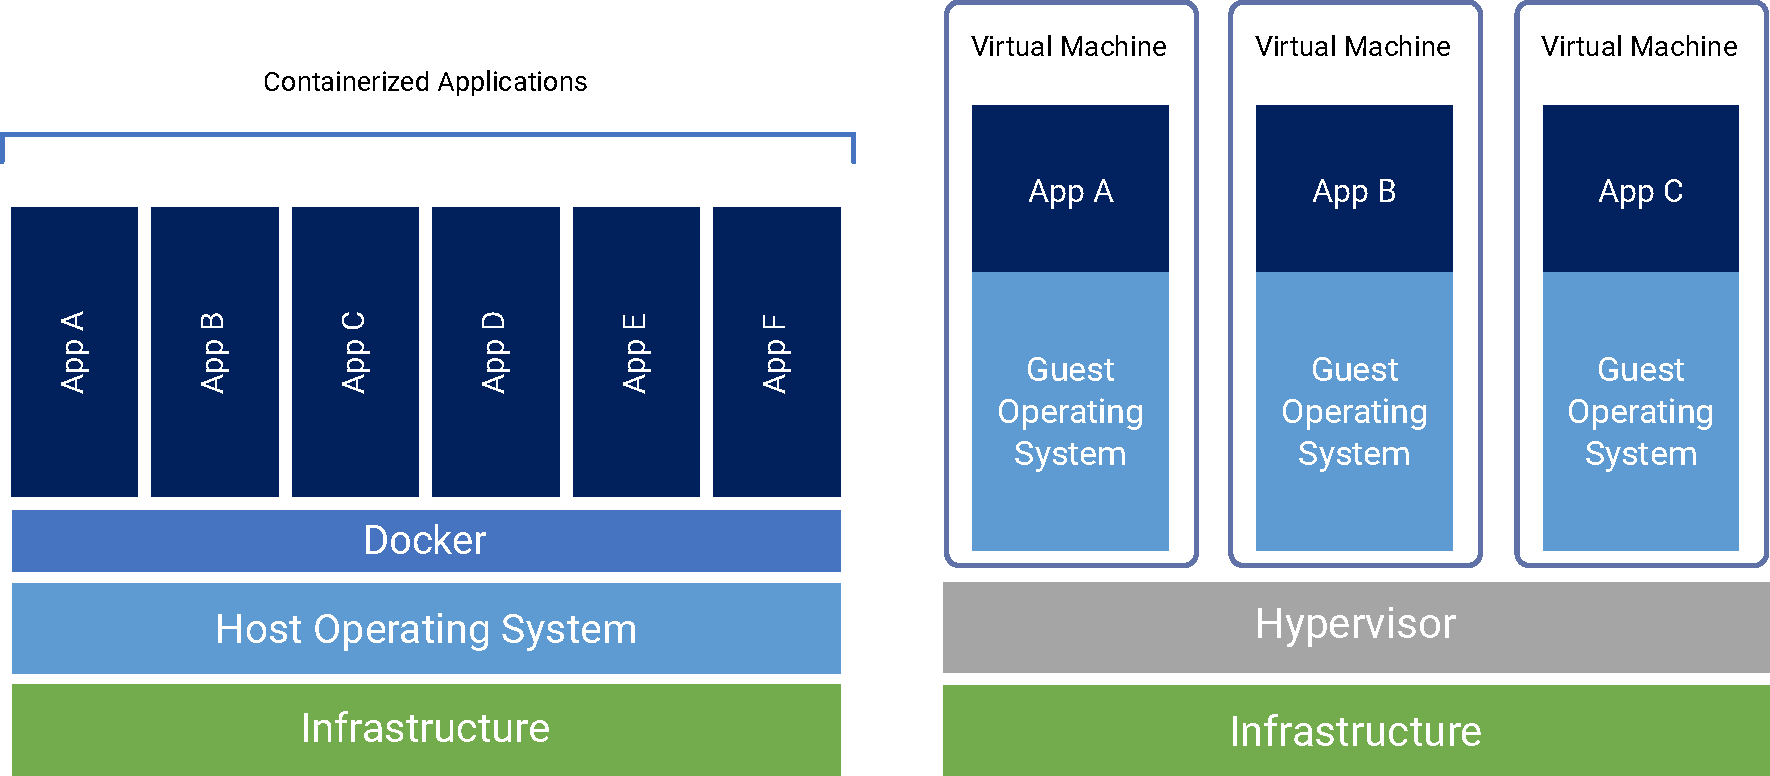
\includegraphics[width=\textwidth]{res/img/Container_vs_Virtual_Host.pdf}
  \caption{Gegenüberstellung der Aufbauweise von Containern (links) und virtuellen Servern (rechts) \parencite{fong2018containervsvirtualhosts}}
  \label{fig:container_vs_virtual_host}
\end{figure}

Wie die \autoref{fig:container_vs_virtual_host} zeigt, braucht die \gls{ac-vm} eine Hardware-Infrastruktur-Ebene, auf der diese aufgebaut werden kann. Darauf wird ein \emph{Hypervisor} bereitgestellt, der als Monitor für die virtuellen Maschinen dient, die auf dem System installiert werden. Es gibt zwei Typen von Virtualisierung. Der erste Typ wird in der Abbildung gezeigt. In dieser stellt der Hypervisor gleichzeitig die Betriebssystemfunktionalität und die VM-Versorgung dar. Typ-2 injiziert zwischen Hypervisor und Infrastruktur ein Betriebssystem, auf dem der Hypervisor läuft. Dies beeinflusst allerdings die Performance von VMs, da dadurch mehr als nur die für den Hypervisor nötigen Betriebssystemfunktionalitäten angesteuert werden. Typ-2 wird dadurch oftmals für die Entwicklung genutzt, während Typ-1 für die tatsächliche Distribution von Software eingesetzt wird. Ein Beispiel für eine Typ-1 Virtualisierung bietet der Hypervisor \emph{ESXi} der Firma \emph{VMware}. Auf dem Hypervisor wird für jede Applikation eine virtuelle Maschine aufgesetzt, die ein eigenes Betriebssystem bereitstellt, auf der die Applikation installiert werden kann. Für den Fall, dass Linux als Betriebssystem gewählt wird, bekäme jede Applikation somit seinen eigenen Linux Kernel. Dies bedeutet im Umkehrschluss, dass jede virtuelle Maschine seinen eigenen Speicherslot bekommt und somit von anderen virtuellen Maschinen isoliert ist. Hinzu kommt, dass jede virtuelle Maschine auch komplett einzeln konfiguriert werden muss. Auch wenn sich \gls{ac-vm}s über die Zeit bewährt und weiterentwickelt haben, bieten Container einige weitere Vorteile \parencites{chelladhurai2017learning}{kane2018docker}.

Container benutzen anders als \acrshort{ac-vm}s keinen Hypervisor, der Funktionalitäten eines Betriebssystems bereitstellt. Stattdessen laufen Container auf einem einzigen Betriebssystem. Container sind somit nur einzelne Prozesse, die allerdings durch \emph{namespaces} und \emph{interne Netzwerke} voneinander isoliert werden. Dies nennt man auch \glqq operating system virtualization \grqq{} \parencite{kane2018docker}. Anders als in \autoref{fig:container_vs_virtual_host} dargestellt laufen Container nicht auf einer Docker Instanz, sondern direkt auf dem Betriebssystem, das bereitgestellt wird. Docker ist dabei ein Werkzeug, womit sich diese Prozesse verwalten lassen. Hierbei ist wichtig darauf zu achten, dass Container nur Applikationen betreiben können, die auch auf dem geteilten Kernel laufen können. Ein Linux Betriebssystem lässt also Container einen Linux Kernel teilen, wodurch Linux Container entstehen. Ein Windows Betriebssystem erstellt demnach Windows basierte Container. Ein Container braucht durch das Teilen des Kerns eines Betriebssystems für jede isolierte Arbeitslast kein komplettes Betriebssystem, wodurch die Installations- und Startzeit von Containern deutlich reduziert wird. Kane und Matthias benennen bei VMs folgendes Problem: \glqq In a VM, calls by the process to the hardware or hypervisor would require bouncing in and out of privileged mode on the processor twice, thereby noticeably slowing down many calls\grqq{} \parencite{kane2018docker}. Das Wegfallen einer Hypervisor-Ebene bei Containern impliziert, dass eine zusätzliche Indirektion beim Ausführen von Applikationen wegfällt, wodurch Container an Performance gewinnen und somit für Microservices in Verbindung mit \gls{ac-cicd} in Frage kommen. Microservices ermöglichen dadurch ein schnelles und mehrmals am Tag erfolgendes Updaten, Kompilieren und Installieren, um Systemfehler auf schnellstmöglichem Weg zu eliminieren \parencites{kane2018docker}{chelladhurai2017learning}.

\begin{figure}[ht!]
  \vspace{.02\textheight}
  \centering
    \begin{tikzpicture}
      \begin{axis}[
        xbar,
        nodes near coords,
        legend style={at={(0.5,-0.15)},anchor=north,legend columns=-1},
        y label style={at={(axis description cs:-.25,.5)},anchor=north},
        width=\textwidth-3.5cm,
        height=5cm,
        scale only axis,
        ylabel=Cloud Computing Systeme,
        xlabel=Anteil der Befragten (\%),
        xmajorgrids,
        xmin=0,
        xmax=100,
        symbolic y coords={Cloud Foundry,Xen,KVM,OpenShift,OpenStack,Kubernetes,Docker},
        y tick label style={rotate=35,anchor=east},
        ytick=data
        ]
        \addplot [color=blue, fill=blue!50, mark=none] table [x=perc, y=ord, col sep=comma] {res/data/statista/open_source_cloud_computing_systems.csv};
      \end{axis}
    \end{tikzpicture}
  \caption{Unter 91 Schweizer Unternehmen durchgeführte Umfrage zur Verwendung von Open Source Cloud Computing Systemen \parencite{stürmer2018cloudcomputing}}
  \label{fig:cloud_computing_systems}
\end{figure}

\autoref{fig:cloud_computing_systems} zeigt eine Statistik aus dem Jahr 2018. Die Statistik war eine Umfrage zu dem Thema, welche Open Source Cloud Computing Systeme in den Organisationen verwendet werden. Dabei wird allerdings nicht nur Container-Software, sondern auch Software für \gls{ac-vm}s betrachtet. Dazu wurden $91$ Schweizer Unternehmen befragt. Docker ist dabei mit einem Vorsprung von $57,1\%$ vor Kubernetes. Dabei muss herausgestellt werden, dass Docker eine Container-Plattform ist, während Kubernetes ein Container-Orchestrierer ist und somit Docker ergänzt. Kubernetes ist das Pendant zu Docker-Swarm, dem hauseigenen Container-Orchestrierer von Docker.

Durch die, wie in \autoref{fig:cloud_computing_systems} beschriebene, hohe Beliebtheit von Docker, wird diese Container-Plattform in dieser Arbeit zum Installieren und Entwickeln von container-basierten Microservices benutzt. Die hohe Verwendungsanzahl von Docker lässt darauf schließen, dass es für diese Software am meisten Unterstützung in Form von Hinweisen, Lösungsvorschlägen und Werkzeugen gibt, was die Wartbarkeit und somit die Zuverlässigkeit des gesamten Systems erhöht. Gleichzeitig können mithilfe von Werkzeugen wie Kubernetes oder Docker-Swarm weitere Vorteile wie dynamische Skalierung von Services genutzt werden.
